\documentclass[12pt,a4paper]{article}
\usepackage[utf8]{inputenc}
\usepackage[english]{babel}			% Encoding
\usepackage{amsmath}
\usepackage{amsfonts}
\usepackage{amssymb}
\usepackage{graphicx}
\usepackage{bbold}
\usepackage{multirow,multicol}
\usepackage{pifont,hyperref,lastpage,fancyhdr,movie15,float}
\usepackage{eqnarray}
\usepackage{geometry}
\usepackage{caption}
\usepackage{subcaption}
\usepackage{pdfpages}
\geometry{a4paper, total={170mm,257mm}, left=20mm, top=20mm,}

%%%%%%%%%%%%%%%%%%%%%%%%%%%%%%%%%%%%%%%%%%%%%%%%%%%%%%%%%%%%%%%%%%%%%%%%%%%%%%%%%%%%%
%%%%%%%%%%%%%%%%%%%%%%%%% FOOTER AND HEADER (DO NOT EDIT) %%%%%%%%%%%%%%%%%%%%%%%%%%%
\pagestyle{fancy}                                                     				%
\fancyhf{} 		                                                     				%
\lfoot{\tiny\textsf{
\includegraphics[width=1.9cm]{Figures/AIMSCameroonlogo}         %
		Po.Box~608 Limbe,~phone~{(+237) 233333363},~                          				%
		\url{http://www.aims-cameroon.org}}}                                  				%
\rfoot{\bfseries Page \thepage~of \pageref{LastPage}}                 				%
\renewcommand{\footrulewidth}{2.pt}\renewcommand{\headrulewidth}{0pt} 				%
%%%%%%%%%%%%%%%%%%%%%%%%% DO NOT EDIT ANYTHING HERE %%%%%%%%%%%%%%%%%%%%%%%%%%%%%%%%%
%%%%%%%%%%%%%%%%%%%%%%%%%%%%%%%%%%%%%%%%%%%%%%%%%%%%%%%%%%%%%%%%%%%%%%%%%%%%%%%%%%%%%


%%%%%%%% FILL HERE INFORMATION ABOUT THE PRESENT ASSIGNMENT %%%%%%%%%%%%%%%%%%%%%%%
\newcommand{\code}{\textbf{rXRB31w8}}                                      %
\newcommand{\deadline}{29.01.22, 6:00 am pm}                                        %
\newcommand{\assignment}{assignment 2 ON "Maths of Quantum Computing"}				           	  % 
\newcommand{\lecturer}{Lecturer(s): "\textbf{Wolfgang Sherer}"}                   		  %
%%%%%%%%%%%%%%%%%%%%%%%%%%%%%%%%%%%%%%%%%%%%%%%%%%%%%%%%%%%%%%%%%%%%%%%%%%%%%%%%%%%

%%%%%%%%%%%%% Title at the first page %%%%%%%%%%%%%%%%%%%%%%%%%%%%%%%%%%%%%%%%%%%%%%%%%%%
\title{\vspace*{-2cm}\begin{minipage}{\textwidth}                                       %
		\begin{center}                                                                          %
			\begin{tabular}{|c|c|c|}                                                                %
				\hline\multicolumn{3}{|c|}{\bf\scriptsize\MakeUppercase\assignment}\\                   %
				\hline{\small Student's Code}&                                                          %
				\multirow{3}{7cm}{
\includegraphics[width=7.1cm,height=1.4cm]{Figures/AIMSCameroonlogo}} %
				& {\small Deadline}\\                                                                   %
				\cline{1-1}\cline{3-3}{\small\bf\code}&&{\small\bf\deadline} \\       					%
				\cline{1-1}\cline{3-3}{\small\today} &&{\small Ac. Year: 2021 - 2022}\\           					%
				\hline\multicolumn{3}{|r|}{\scriptsize\lecturer}\\\hline              					%
			\end{tabular}                                                         					%
		\end{center}                                                          					%
	\end{minipage}\hfill\date{}\vspace*{-1cm}}                            					%
%%%%%%%%%%%%%%%%%%%%%%%%%%%%%%%%%%%%%%%%%%%%%%%%%%%%%%%%%%%%%%%%%%%%%%%%%%%%%%%%%%%%%%%%%

\newcommand{\K}{\mathbb{K}}
\newcommand{\R}{\mathbb{R}}
\newcommand{\C}{\mathbb{C}}
\newcommand{\D}{\mathbb{D}}
\newcommand{\Z}{\mathbb{Z}}
\newcommand{\N}{\mathbb{N}}


\newtheorem{theo}{Theorem}
\newtheorem{defi}{Definition}
\newtheorem{prop}{Proposition}
\newenvironment{proof}[1][Proof.]{\textbf{#1~}}{\ \rule{0.5em}{0.5em}}
%%%%%%%%%%%%%%%%%%%%�tensor product%%%%%%%%%%%%%%%%%%%%%
\newcommand{\tket}[2]{|#1\rangle\otimes|#2\rangle}
\newcommand{\tbra}[2]{\langle#1|\otimes\langle#2|}
\newcommand{\tpro}[2]{|#1\rangle\otimes\langle#2|}

%%%%%%%%%%%%%%%%%%%%%%%Shorcut commands%%%%%%%%%%%%%%%%%%%%%%%%%%%%%%%%%
\newcommand{\no}[1]{||#1||}
\newcommand{\ket}[1]{|#1\rangle}
\newcommand{\bra}[1]{\langle #1 |}
\newcommand{\av}[1]{\langle{#1}\rangle} %Average
\newcommand{\avp}[1]{\langle{#1}\rangle_{\psi}}
\newcommand{\kb}[2]{|#1\rangle\langle#2|} %ketbra
\newcommand{\proj}[1]{\ket{#1}\bra{#1}} % Projecteur
\newcommand{\bk}[2]{\langle#1\ket{#2}} %braket
\newcommand{\mel}[3]{\bra{#1}#2\ket{#3}} %Matrix element
\newcommand{\ep}{\hat{e}_p} 
\newcommand{\fq}{\hat{f}_q} 
\newcommand{\ddt}[1]{\frac{\mathrm{d}#1}{\mathrm{d}t}} 
\newcommand\norm[1]{\lVert#1\rVert}
\newcommand{\X}{\mathtt{X}} 
\newcommand{\HH}{\mathtt{H}} 
\newcommand{\I}{\mathbb{I}} 
\newcommand{\kup}{|\uparrow_{\vec{\hat{n}}}\rangle} 
\newcommand{\pup}{|\downarrow_{\vec{\hat{n}}}\rangle}
\newcommand{\bup}{\langle\uparrow_{\hat{n}} |} 
\newcommand{\hpsi}{\hat{\Psi}_{pq}}
\newcommand{\hphi}{\hat{\Phi}_{pq}}
\newcommand{\six}{\sigma_x}
\newcommand{\siy}{\sigma_y}
\newcommand{\siz}{\sigma_z}


\newcommand{\eqt}[1]
{\begin{equation}#1
\end{equation}}


%%%%%%%%%%%%%%%%%%Shorcut for the imbrication between environemnt equation and thet environment split%%%%%%%%%%%%%%%%%
\newcommand{\eqtt}[1]
{\begin{equation} \begin{split}#1
\end{split}\end{equation}}

\newcommand{\eqalign}[1]
{ \begin{align}#1
\end{align}}

\newcommand{\eqtta}[1]
{\begin{equation} \left\{\begin{split}#1
	\end{split}\end{equation}\right. }


\begin{document}
\maketitle\thispagestyle{fancy}

\section*{Exercise 1}
\begin{enumerate}
\item Using the \textbf{NOT-gate} $\X$, the Hadamard gate $\HH$ and the \textbf{C.NOT} get $\Lambda^1(\X)$ build a circuit \eqt{U: {}^\mathrm{q}\mathcal{H}^{\otimes2}\rightarrow {}^\mathrm{q}\mathcal{H}^{\otimes2}.}
\eqt{U\ket{00}=\ket{\Psi^+}.}
\begin{itemize}
	\item \textbf{Step 1}\\
	We apply the gate $\X$ on the second qubit and the identity to the first qubit. We have:
	\eqtt{
	(\mathbb{I}\otimes \X)\ket{00}&=\mathbb{I}\ket{0}\otimes \X\ket{0},\\
	&=\ket{0}\otimes\ket{1}.}
		\item \textbf{Step 2}\\
		We apply the Hadamard operator $\HH\otimes1$ on the result of the first step to obtain :
		\eqtt{
	\HH\otimes \I\ket{01}&=\HH\ket{0}\otimes\ket{1},\\
		&=\frac{1}{\sqrt{2}}(\ket{0}+\ket{1})\otimes\ket{1}	, \text{ since } \HH\ket{0}=\frac{1}{\sqrt{2}}(\ket{0}+\ket{1}),\\
		&=\frac{1}{\sqrt{2}}(\ket{01}+\ket{11}).
	}
				\item \textbf{Step 3}\\		
		We apply the \textbf{CNOT-gate}. The operator $\Lambda^1(\X)$ is a 2-qubit gate such that when it is applied, the second qubit is flipped when the first qubit is the state 1, and remains the same when the first qubit is in the state 0.\\
	So we have that:
	\eqtt{
	\Lambda^1(\X)\frac{1}{\sqrt{2}}(\ket{01}+\ket{11})&=\frac{1}{\sqrt{2}}\left(\Lambda^1 (\X)\ket{01}+\Lambda^1(\X)\ket{11} \right)\\ 
	&=\frac{1}{\sqrt{2}}\ket{01}+\ket{10}\\
	&=\ket{\Psi^+}.}
\end{itemize}
\begin{figure}[!h]
	\centering
	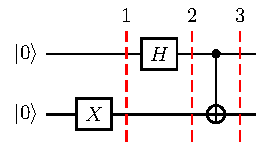
\includegraphics[scale=1.5]{Figures/circuit}
	\caption{Quantum circuit U}
\end{figure}
\newpage
\item We give the matrix $U$ in the computational basis:
\eqt{U=\Lambda^1 (\X)\left( \HH\otimes\mathbb{\I}\right) \left(\I\otimes \X \right).}
We have:
\eqt{
\I\otimes \X =
\begin{pmatrix}
	1.\X&0\X\\
	0.\X&1.\X
\end{pmatrix}
=
\begin{pmatrix}
	1.\begin{pmatrix} 0&1\\0&1\end{pmatrix}&0.\begin{pmatrix} 0&1\\0&1\end{pmatrix}\\
	0.\begin{pmatrix} 0&1\\0&1\end{pmatrix}&1.\begin{pmatrix} 0&1\\0&1\end{pmatrix}
\end{pmatrix}
=
\begin{pmatrix}
0&1&0&0\\
1&0&0&0\\
0&0&0&1\\
0&0&1&0
\end{pmatrix}.}
Also, 
\eqtt{
\HH\otimes\I &=\frac{1}{\sqrt{2}} \begin{pmatrix}
1&1\\
1&-1
\end{pmatrix}\otimes\begin{pmatrix}
1&0\\
0&1
\end{pmatrix},\\
&=\frac{1}{\sqrt{2}} \begin{pmatrix}
1.\I&1.\I\\
1.\I&-1.\I
\end{pmatrix}\\&=\frac{1}{\sqrt{2}}\begin{pmatrix}1.\begin{pmatrix}
1&0\\
0&1
\end{pmatrix}&
1.\begin{pmatrix}
1&0\\
0&1
\end{pmatrix}\\1.\begin{pmatrix}
1&0\\
0&1
\end{pmatrix}&
-1.\begin{pmatrix}
	1&0\\
	0&1
\end{pmatrix}\end{pmatrix}\\
&=\frac{1}{\sqrt{2}} \begin{pmatrix}
1&0&1&0\\
0&1&0&1\\
1&0&-1&0\\
0&1&0&-1
\end{pmatrix}}
And,
\begin{align*}
\Lambda^1(\X)&=\ket{0}\bra{0}\otimes\I+\ket{1}\bra{1}\otimes \X,\\\\
&=\begin{pmatrix}
1&0\\
0&0
\end{pmatrix}\otimes\I+\begin{pmatrix}
0&0\\
0&1
\end{pmatrix}\otimes \X,\\\\
&=\begin{pmatrix}
1&0&0&0\\
0&1&0&0\\
0&0&0&0\\
0&0&0&0
\end{pmatrix}+\begin{pmatrix}
0&0&0&0\\
0&0&0&0\\
0&0&0&1\\
0&0&1&0
\end{pmatrix},\\\\
&=\begin{pmatrix}
1&0&0&0\\
0&1&0&0\\
0&0&0&1\\
0&0&1&0
\end{pmatrix}.
\end{align*}
Now given that: \eqt{U=\Lambda^1(X)\left( \HH\otimes\I\right)\left(\I\otimes \X \right).}
Then we have that:
\eqtt{
U&=\frac{1}{\sqrt{2}}\begin{pmatrix}
0&1&0&0\\
1&0&0&0\\
0&0&0&1\\
0&0&1&0
\end{pmatrix}\begin{pmatrix}
1&0&1&0\\
0&1&0&1\\
1&0&-1&0\\
0&1&0&-1
\end{pmatrix}\begin{pmatrix}
0&1&0&0\\
1&0&0&0\\
0&0&0&1\\
0&0&1&0
\end{pmatrix},\\\\
&=\frac{1}{\sqrt{2}}\begin{pmatrix}
0&1&0&0\\
1&0&0&0\\
0&0&0&1\\
0&0&1&0
\end{pmatrix}\begin{pmatrix}
0&1&0&1\\
1&0&1&0\\
0&1&0&-1\\
1&0&-1&0
\end{pmatrix},\\\\
&=\frac{1}{\sqrt{2}}\begin{pmatrix}
0&1&0&1\\
1&0&1&0\\
1&-1&0&1\\
0&1&0&-1
\end{pmatrix}.
}
%
Therefore the matrix $U$ in the computational basis is given by:
\eqt{U=\frac{1}{\sqrt{2}}\begin{pmatrix}
0&1&0&1\\
1&0&1&0\\
1&-1&0&1\\
0&1&0&-1
\end{pmatrix}.}
\item See Python code. 
\item See Python code 
%
\item Show that the result is indeed $\ket{\Psi^+}$.\\
The state vector obtained obtained while programming on qiskit is
\eqt{\begin{pmatrix}
	0\\
	\frac{1}{\sqrt{2}}\\
	\frac{1}{\sqrt{2}}\\
	0
\end{pmatrix}.}
$\ket{\Psi^+}$ is given by:
\eqtt{
	\ket{\Psi^+}&=\frac{1}{\sqrt{2}}\left( \ket{01}+\ket{10}\right) \\
	&=\frac{1}{\sqrt{2}}\left( \ket{0}\otimes\ket{1}+\ket{1}\otimes\ket{0}\right)\\
	&=\frac{1}{\sqrt{2}} \left(\begin{pmatrix}
		1\\
		0
	\end{pmatrix}\otimes\begin{pmatrix}
		0\\
		1
	\end{pmatrix}+\begin{pmatrix}
		0\\
		1
	\end{pmatrix}\otimes\begin{pmatrix}
		1\\
		0
	\end{pmatrix}\right)}
\eqtt{
	\ket{\Psi^+}&=\frac{1}{\sqrt{2}}(\ket{01}+\ket{10})\\&=\frac{1}{\sqrt{2}}\begin{pmatrix}
		1.\begin{pmatrix}
			0\\
			1
		\end{pmatrix}\\
		0.\begin{pmatrix}
			0\\
			1\end{pmatrix}\end{pmatrix}+\frac{1}{\sqrt{2}}\begin{pmatrix}
		0.\begin{pmatrix}
			1\\
			0
		\end{pmatrix}\\
		1.\begin{pmatrix}
			1\\
			0
	\end{pmatrix} \end{pmatrix}\\
	&=\frac{1}{\sqrt{2}}\left(\begin{pmatrix}
		0\\
		1\\
		0\\
		0
	\end{pmatrix}+\begin{pmatrix}
		0\\
		0\\
		1\\
		0
	\end{pmatrix}\right)\\
	&=\begin{pmatrix}
		0\\
		\frac{1}{\sqrt{2}}\\
		\frac{1}{\sqrt{2}}\\
		0
	\end{pmatrix}=\ket{\Psi^+}.}
Hence, the result obtained is indeed $\ket{\Psi^+}.$
\end{enumerate}

\end{document}
